% %% %%%%%%%%%%%%%%%%%%%%%%%%%%%%%%%%%%%%%%%%%%%%%%%%%%%%%%%%%
%
% reporte.tex
%
%  Author: Mauricio Matamoros
%  Date:   2020.02.28
%
%  Ejemplo de reporte escrito para práctica de laboratorio
%
% %% %%%%%%%%%%%%%%%%%%%%%%%%%%%%%%%%%%%%%%%%%%%%%%%%%%%%%%%%%
% La raiz del proyecto (este archivo)
%!TEX root = ./reporte.tex
% Archivo de referencias bibliográficas
%!TEX root = ./references.bib

% CHKTEX-FILE 1
% Plantilla de artículo con fuente de 10.5 puntos a doble columna en papel tamaño carta
\documentclass[letterpaper,10.5pt,twocolumn]{article}
% Plantilla de artículo con fuente de 10.5 puntos en papel tamaño carta
% \documentclass[letterpaper,10.5pt]{article}

% Configurado el tipo de documento, se agregan los paquetes
% %% %%%%%%%%%%%%%%%%%%%%%%%%%%%%%%%%%%%%%%%%%%%%%%%%%%%%%%%%%
%
% packages.tex
%
%  Author: Mauricio Matamoros
%  Date:   2020.02.28
%
%  Contiene la lista de paquetes requeridos para generar
%  el archivo-reporte de las prácticas de laboratorio
%
% %% %%%%%%%%%%%%%%%%%%%%%%%%%%%%%%%%%%%%%%%%%%%%%%%%%%%%%%%%%
% Archivo principal de LaTeX
%!TEX root = ../reporte.tex

\usepackage[utf8]{inputenc}                  % Soporte para utf8
\usepackage[T1]{fontenc}                     % Soporte extendido de caracteres unicode
\usepackage[english,spanish,mexico]{babel}   % Define el idioma del documento a español (México) con soporte para inglés
% Standard packages
\usepackage{float}                           % Imágenes flotantes en el documento
\usepackage{ifthen}                          % Soporte if-then en macros
\usepackage{xspace}                          % Soporte de autoespaciado en macros
\usepackage{xstring}                         % Operaciones con cadenas en macros
\usepackage{wrapfig}                         % Permite colocar texto al rededor de figuras y otros flotantes
\usepackage{booktabs}                        % Embellece tablas
\usepackage{csquotes}                        % Entrecomillado automático y manejo de citas textuales
\usepackage{fancyhdr}                        % Permite reconfigurar encabezado y pie de página
\usepackage{fancyvrb}                        % Define estilos para entornos Verbatim
\usepackage{geometry}                        % Permite reconfigurar la geometría del documento
\usepackage{graphicx}                        % Permite insertar imágenes en varios formatos
\usepackage{lastpage}                        % Referencia a la última página del documento
\usepackage{listings}                        % Define estilos para entornos de código de programación (sintaxis)
\usepackage{multicol}                        % Manejo de texto en varias columnas
\usepackage{tabularx}                        % Tablas con ancho de columna variable
\usepackage{algorithm}                       % Entorno para escribir algoritmos
\usepackage{algpseudocode}                   % Entorno para escribir algoritmos en pseudocódigo
\usepackage[justification=centering]{subcaption} % Permite imágenes en viñetas
\usepackage[all]{nowidow}                    % Control de viudas y huérfanas
\usepackage[inline]{enumitem}                % Añade opciones de configuración a listas
\usepackage[usenames,dvipsnames]{xcolor}     % Permite el uso de colores en el documento
% Referencing
\usepackage{varioref}                        % Gestión de referencias variables
\usepackage{hyperref}                        % Gestión de referencias e hipervínculos
\usepackage[noabbrev,nameinlink,spanish]{cleveref} % Gestión de referencias cruzadas inteligentes con hipervínculos
\usepackage[square, comma, numbers, sort&compress]{natbib} % Gestión de referencias bibliográficas


% Tras los paquetes se añaden las macros (nuevas funciones)

\newcommand{\lpar}{(}\newcommand{\rpar}{)} %CHKTEX 9
\newcommand{\IIC}{I\textsuperscript{2}C\xspace}
\newcommand{\GND}{\textsc{Gnd}\xspace}
\newcommand{\VCC}{\textsc{Vcc}\xspace}
\newcommand{\VDD}{\textsc{Vdd}\xspace}
\newcommand{\textbi}[1]{\textbf{\textit{#1}}}
\newcommand{\degreesC}[1]{%
	#1\textsuperscript{o}C\xspace{}%
}
\newcommand{\degreesF}[1]{%
	#1\textsuperscript{o}F\xspace{}%
}

% \newcommand{\VCC}{V\textsubscript{CC}\xspace{}}
% \newcommand{\GND}{\textsc{Gnd}\xspace{}}

% Escriba a continuación el título del documento y su nombre
\author{Fulano de Tal} % Su nombre
\title{Práctica N. \enquote{Título de la Práctica}} % Título del documento
% \date{} % Fecha de creación del documento


% A continuacion se configura la página y la geometría del documento
% CHKTEX-FILE 1
% CHKTEX-FILE 13
% CHKTEX-FILE 18
% CHKTEX-FILE 35
\documentclass[letterpaper,12pt,twocolumn]{article}
% Input encodign

% %% %%%%%%%%%%%%%%%%%%%%%%%%%%%%%%%%%%%%%%%%%%%%%%%%%%%%%%%%%
%
% packages.tex
%
%  Author: Mauricio Matamoros
%  Date:   2020.02.28
%
%  Contiene la lista de paquetes requeridos para generar
%  el archivo-reporte de las prácticas de laboratorio
%
% %% %%%%%%%%%%%%%%%%%%%%%%%%%%%%%%%%%%%%%%%%%%%%%%%%%%%%%%%%%
% Archivo principal de LaTeX
%!TEX root = ../reporte.tex

\usepackage[utf8]{inputenc}                  % Soporte para utf8
\usepackage[T1]{fontenc}                     % Soporte extendido de caracteres unicode
\usepackage[english,spanish,mexico]{babel}   % Define el idioma del documento a español (México) con soporte para inglés
% Standard packages
\usepackage{float}                           % Imágenes flotantes en el documento
\usepackage{ifthen}                          % Soporte if-then en macros
\usepackage{xspace}                          % Soporte de autoespaciado en macros
\usepackage{xstring}                         % Operaciones con cadenas en macros
\usepackage{wrapfig}                         % Permite colocar texto al rededor de figuras y otros flotantes
\usepackage{booktabs}                        % Embellece tablas
\usepackage{csquotes}                        % Entrecomillado automático y manejo de citas textuales
\usepackage{fancyhdr}                        % Permite reconfigurar encabezado y pie de página
\usepackage{fancyvrb}                        % Define estilos para entornos Verbatim
\usepackage{geometry}                        % Permite reconfigurar la geometría del documento
\usepackage{graphicx}                        % Permite insertar imágenes en varios formatos
\usepackage{lastpage}                        % Referencia a la última página del documento
\usepackage{listings}                        % Define estilos para entornos de código de programación (sintaxis)
\usepackage{multicol}                        % Manejo de texto en varias columnas
\usepackage{tabularx}                        % Tablas con ancho de columna variable
\usepackage{algorithm}                       % Entorno para escribir algoritmos
\usepackage{algpseudocode}                   % Entorno para escribir algoritmos en pseudocódigo
\usepackage[justification=centering]{subcaption} % Permite imágenes en viñetas
\usepackage[all]{nowidow}                    % Control de viudas y huérfanas
\usepackage[inline]{enumitem}                % Añade opciones de configuración a listas
\usepackage[usenames,dvipsnames]{xcolor}     % Permite el uso de colores en el documento
% Referencing
\usepackage{varioref}                        % Gestión de referencias variables
\usepackage{hyperref}                        % Gestión de referencias e hipervínculos
\usepackage[noabbrev,nameinlink,spanish]{cleveref} % Gestión de referencias cruzadas inteligentes con hipervínculos
\usepackage[square, comma, numbers, sort&compress]{natbib} % Gestión de referencias bibliográficas


\newcommand{\lpar}{(}\newcommand{\rpar}{)} %CHKTEX 9
\newcommand{\IIC}{I\textsuperscript{2}C\xspace}
\newcommand{\GND}{\textsc{Gnd}\xspace}
\newcommand{\VCC}{\textsc{Vcc}\xspace}
\newcommand{\VDD}{\textsc{Vdd}\xspace}
\newcommand{\textbi}[1]{\textbf{\textit{#1}}}
\newcommand{\degreesC}[1]{%
	#1\textsuperscript{o}C\xspace{}%
}
\newcommand{\degreesF}[1]{%
	#1\textsuperscript{o}F\xspace{}%
}

% \newcommand{\VCC}{V\textsubscript{CC}\xspace{}}
% \newcommand{\GND}{\textsc{Gnd}\xspace{}}
% CHKTEX-FILE 1
% CHKTEX-FILE 13
% CHKTEX-FILE 18
% CHKTEX-FILE 35
\documentclass[letterpaper,12pt,twocolumn]{article}
% Input encodign

% %% %%%%%%%%%%%%%%%%%%%%%%%%%%%%%%%%%%%%%%%%%%%%%%%%%%%%%%%%%
%
% packages.tex
%
%  Author: Mauricio Matamoros
%  Date:   2020.02.28
%
%  Contiene la lista de paquetes requeridos para generar
%  el archivo-reporte de las prácticas de laboratorio
%
% %% %%%%%%%%%%%%%%%%%%%%%%%%%%%%%%%%%%%%%%%%%%%%%%%%%%%%%%%%%
% Archivo principal de LaTeX
%!TEX root = ../reporte.tex

\usepackage[utf8]{inputenc}                  % Soporte para utf8
\usepackage[T1]{fontenc}                     % Soporte extendido de caracteres unicode
\usepackage[english,spanish,mexico]{babel}   % Define el idioma del documento a español (México) con soporte para inglés
% Standard packages
\usepackage{float}                           % Imágenes flotantes en el documento
\usepackage{ifthen}                          % Soporte if-then en macros
\usepackage{xspace}                          % Soporte de autoespaciado en macros
\usepackage{xstring}                         % Operaciones con cadenas en macros
\usepackage{wrapfig}                         % Permite colocar texto al rededor de figuras y otros flotantes
\usepackage{booktabs}                        % Embellece tablas
\usepackage{csquotes}                        % Entrecomillado automático y manejo de citas textuales
\usepackage{fancyhdr}                        % Permite reconfigurar encabezado y pie de página
\usepackage{fancyvrb}                        % Define estilos para entornos Verbatim
\usepackage{geometry}                        % Permite reconfigurar la geometría del documento
\usepackage{graphicx}                        % Permite insertar imágenes en varios formatos
\usepackage{lastpage}                        % Referencia a la última página del documento
\usepackage{listings}                        % Define estilos para entornos de código de programación (sintaxis)
\usepackage{multicol}                        % Manejo de texto en varias columnas
\usepackage{tabularx}                        % Tablas con ancho de columna variable
\usepackage{algorithm}                       % Entorno para escribir algoritmos
\usepackage{algpseudocode}                   % Entorno para escribir algoritmos en pseudocódigo
\usepackage[justification=centering]{subcaption} % Permite imágenes en viñetas
\usepackage[all]{nowidow}                    % Control de viudas y huérfanas
\usepackage[inline]{enumitem}                % Añade opciones de configuración a listas
\usepackage[usenames,dvipsnames]{xcolor}     % Permite el uso de colores en el documento
% Referencing
\usepackage{varioref}                        % Gestión de referencias variables
\usepackage{hyperref}                        % Gestión de referencias e hipervínculos
\usepackage[noabbrev,nameinlink,spanish]{cleveref} % Gestión de referencias cruzadas inteligentes con hipervínculos
\usepackage[square, comma, numbers, sort&compress]{natbib} % Gestión de referencias bibliográficas


\newcommand{\lpar}{(}\newcommand{\rpar}{)} %CHKTEX 9
\newcommand{\IIC}{I\textsuperscript{2}C\xspace}
\newcommand{\GND}{\textsc{Gnd}\xspace}
\newcommand{\VCC}{\textsc{Vcc}\xspace}
\newcommand{\VDD}{\textsc{Vdd}\xspace}
\newcommand{\textbi}[1]{\textbf{\textit{#1}}}
\newcommand{\degreesC}[1]{%
	#1\textsuperscript{o}C\xspace{}%
}
\newcommand{\degreesF}[1]{%
	#1\textsuperscript{o}F\xspace{}%
}

% \newcommand{\VCC}{V\textsubscript{CC}\xspace{}}
% \newcommand{\GND}{\textsc{Gnd}\xspace{}}
% CHKTEX-FILE 1
% CHKTEX-FILE 13
% CHKTEX-FILE 18
% CHKTEX-FILE 35
\documentclass[letterpaper,12pt,twocolumn]{article}
% Input encodign

\input{setup/packages}
\input{setup/macros}
\input{setup/document}
\input{setup/listings}

\author{\footnotesize Autor: José Mauricio Matamoros de Maria y Campos}
\title{Especificación para reportes de lectura}
\date{}


% Document body
\begin{document}
\maketitle

\section*{Reportes de lectura}
El objetivo de las lecturas asignadas como tarea es fomentar en el alumno el hábito de la lectura, tanto de documentos técnicos como literarios, ya sean estos en español o en inglés, además de incrementar las habilidades de comprensión de lectura, concreción de ideas, síntesis y redacción de texto en prosa.

Leer es muy importante en el aprendizaje pues la mayor parte de lo que se aprende se hace por medio de la lectura.
Cuando se quiere aprender algo, lo primero que se hace es leer.

Cuando se lee un texto con fines de estudio se resaltan las ideas importantes, se resume, se separan las ideas principales y se formulan cuestionarios para mejor comprender el texto. Cuando se lee por entretenimiento (por ejemplo un cuento o una novela), el texto se analiza y se relacionan hechos y situaciones a fin de poder disfrutar de él.

Un reporte de lectura es un informe escrito acerca del texto que se leyó.
Este informe debe contener los siguientes datos:

\begin{itemize}[noitemsep]
	\item Título del texto y nombre del autor
	\item Tema o asunto que trata
	\item Resumen, síntesis o reseña del texto
	\item Análisis crítico del contenido del texto
	\item Opinión personal del contenido de la lectura
	\item Conclusiones de la lectura
\end{itemize}

En el caso de texto literario no se espera un resumen, síntesis o reseña del texto, sino que deberá comentarse sobre la temática del mismo y resaltar los puntos más importantes, dejando claras sus impresiones y comentarios sobre el texto.

Tome en cuenta que ni la síntesis ni los resúmenes implican copiar y pegar párrafos enteros del texto. Lo importante es distinguir las ideas principales, hacerlas propias y (salvo que sean definiciones), parafrasearlas, es decir,  expresarlas en sus propias palabras.

Pasos para elaborar un reporte de lectura
\begin{enumerate}[noitemsep]
	\item Lea atentamente el texto. Evite distractores como música fuerte, televisión, teléfono, etc.
	\item Anote los términos y palabras que no conozca o entienda e investigue su significado en un diccionario.
	\item Una vez aclarados los términos desconocidos y palabras nuevas, vuelva a leer el texto para comprenderlo mejor.
	\item En la segunda lectura subraye o marque las ideas principales del texto.
	%Procure no escribir en los libros, especialmente si no le pertenecen. Si desea hacer anotaciones, utilice un lápiz blando y escriba con suavidad, o de preferencia use fotocopias.
	\item Tome las ideas principales, abstraígalas, analícelas y sólo entonces redacte su escrito.
\end{enumerate}
\end{document}

%CHKTEX-FILE 1
%CHKTEX-FILE 7
%CHKTEX-FILE 9
% Default fixed font does not support bold face
\DeclareFixedFont{\ttb}{T1}{txtt}{bx}{n}{8} % for bold
\DeclareFixedFont{\ttm}{T1}{txtt}{m}{n}{8}  % for normal

% Custom colors
\usepackage{color}
\definecolor{keywordsColor}{rgb}{0,0,0.5}
\definecolor{customColor}{rgb}{0.6,0,0}
\definecolor{stringColor}{rgb}{0,0.5,0}

% Code highlighting python
\renewcommand{\ttdefault}{pcr}
\lstset{
	language=Python,                              % the language of the code (can be overrided per snippet)
	backgroundcolor=\color{white},                % choose the background color
	basicstyle=\footnotesize\ttfamily,            % the size of the fonts that are used for the code
	breakatwhitespace=false,                      % sets if automatic breaks should only happen at whitespace
	breaklines=true,                              % sets automatic line breaking
	captionpos=t,                                 % sets the caption-position to bottom
	commentstyle=\color{gray},                    % comment style
	deletekeywords={},                            % if you want to delete keywords from the given language
%	escapeinside={\%*}{*)},                       % if you want to add LaTeX within your code
	extendedchars=true,                           % lets you use non-ASCII characters; for 8-bits encodings only, does not work with UTF-8
	frame=tb,                                     % adds a frame around the code
	keepspaces=true,                              % keeps spaces in text, useful for keeping indentation of code (possibly needs columns=flexible)
	keywordstyle=\color{keywordsColor}\bfseries,  % keyword style
	numbers=left,                                 % where to put the line-numbers; possible values are (none, left, right)
	numbersep=5pt,                                % how far the line-numbers are from the code
	numberstyle=\tiny\color{gray},                % the style that is used for the line-numbers
	rulecolor=\color{black},                      % if not set, the frame-color may be changed on line-breaks within not-black text (e.g. comments (green here))
	showspaces=false,                             % show spaces everywhere adding particular underscores; it overrides 'showstringspaces'
	showstringspaces=false,                       % underline spaces within strings only
	showtabs=false,                               % show tabs within strings adding particular underscores
	stepnumber=1,                                 % the step between two line-numbers. If it's 1, each line will be numbered
	stringstyle=\color{stringColor},              % string literal style
	tabsize=2,                                    % sets default tabsize to 2 spaces
	title=\lstname,                               % show the filename of files included with \lstinputlisting; also try caption instead of title
	columns=fixed,                                % Using fixed column width (for e.g. nice alignment)
	otherkeywords={self},                         % if you want to add more keywords to the set
	emphstyle=\color{customColor}\bfseries,       % Custom highlighting style
	emph={__init__,__main__,True,False,None},     % Custom highlighting keywords
	xleftmargin=1cm,                              % Left margin
	xrightmargin=1cm,                             % Right margin
	% Unicode compatibility
	inputencoding=utf8,
	literate={%
	            {Á}{{\'a}}1 {É}{{\'E}}1 {Í}{{\'I}}1 {Ó}{{\'O}}1 {Ú}{{\'U}}1%
	            {á}{{\'a}}1 {é}{{\'e}}1 {í}{{\'i}}1 {ó}{{\'o}}1 {ú}{{\'u}}1%
	            {À}{{\`A}}1 {È}{{\'E}}1 {Ì}{{\`I}}1 {Ò}{{\`O}}1 {Ù}{{\`U}}1%
	            {à}{{\`a}}1 {è}{{\`e}}1 {ì}{{\`i}}1 {ò}{{\`o}}1 {ù}{{\`u}}1%
	            {Ä}{{\"A}}1 {Ë}{{\"E}}1 {Ï}{{\"I}}1 {Ö}{{\"O}}1 {Ü}{{\"U}}1%
	            {ä}{{\"a}}1 {ë}{{\"e}}1 {ï}{{\"i}}1 {ö}{{\"o}}1 {ü}{{\"u}}1%
	            {Â}{{\^A}}1 {Ê}{{\^E}}1 {Î}{{\^I}}1 {Ô}{{\^O}}1 {Û}{{\^U}}1%
	            {â}{{\^a}}1 {ê}{{\^e}}1 {î}{{\^i}}1 {ô}{{\^o}}1 {û}{{\^u}}1% CHKTEX 19
	            {Ã}{{\~a}}1 {Ẽ}{{\~E}}1 {Ĩ}{{\~I}}1 {Õ}{{\~O}}1 {Ũ}{{\~U}}1 {Ñ}{{\~N}}1%
	            {ã}{{\~a}}1 {ẽ}{{\~e}}1 {ĩ}{{\~i}}1 {õ}{{\~o}}1 {ũ}{{\~u}}1 {ñ}{{\~n}}1%
	            {œ}{{\oe}}1 {Œ}{{\OE}}1 {æ}{{\ae}}1 {Æ}{{\AE}}1 {ß}{{\ss}}1%
	            {ç}{{\c c}}1 {Ç}{{\c C}}1 {ø}{{\o}}1 {å}{{\r a}}1 {Å}{{\r A}}1%
	            {€}{{\EUR}}1 {£}{{\pounds}}1 {×}{{\(\times\)}}1% CHKTEX 21
	            {°}{{\textsuperscript{o}}}1%
	            {¹}{{\textsuperscript{1}}}1%
	            {²}{{\textsuperscript{2}}}1%
	            {³}{{\textsuperscript{3}}}1%
	            {⁴}{{\textsuperscript{4}}}1% CHKTEX 19
	            {⁵}{{\textsuperscript{5}}}1% CHKTEX 19
	            {⁶}{{\textsuperscript{6}}}1% CHKTEX 19
	            {⁷}{{\textsuperscript{7}}}1% CHKTEX 19
	            {⁸}{{\textsuperscript{8}}}1% CHKTEX 19
	            {⁹}{{\textsuperscript{9}}}1% CHKTEX 19
	            {⁰}{{\textsuperscript{0}}}1% CHKTEX 19
%	            {A}{{\textAlpha}}1
	            {α}{{\textalpha}}1%
%	            {B}{{\textBeta}}1
	            {β}{{\textbeta}}1%
	            {Γ}{{\textGamma}}1
	            {γ}{{\textgamma}}1%
	            {Δ}{{\textDelta}}1
	            {δ}{{\textdelta}}1% CHKTEX 19
%	            {E}{{\textEpsilon}}1
	            {ϵ}{{\textepsilon}}1%
%	            {Z}{{\textZeta}}1
	            {ζ}{{\textzeta}}1%
%	            {H}{{\textEta}}1
	            {η}{{\texteta}}1%
	            {Θ}{{\textTheta}}1
	            {θ}{{\texttheta}}1%
%	            {I}{{\textIota}}1
	            {ι}{{\textiota}}1%
%	            {K}{{\textKappa}}1
	            {κ}{{\textkappa}}1%
	            {Λ}{{\textLambda}}1
	            {λ}{{\textlambda}}1%
%	            {M}{{\textMu}}1
	            {μ}{{\textmu}}1%
%	            {N}{{\textNu}}1
	            {ν}{{\textnu}}1%
	            {Ξ}{{\textXi}}1
	            {ξ}{{\textxi}}1%
%	            {O}{{\textOmikron}}1
%	            {o}{{\textomikron}}1%
	            {Π}{{\textPi}}1
	            {π}{{\textpi}}1%
%	            {P}{{\textRho}}1
	            {ρ}{{\textrho}}1%
	            {Σ}{{\textSigma}}1
	            {σ}{{\textsigma}}1%
%	            {T}{{\textTau}}1
	            {τ}{{\texttau}}1%
	            {ϒ}{{\textUpsilon}}1
	            {υ}{{\textupsilon}}1%
	            {Φ}{{\textPhi}}1
	            {ϕ}{{\textphi}}1%
%	            {X}{{\textChi}}1
	            {χ}{{\textchi}}1%
	            {Ψ}{{\textPsi}}1
	            {ψ}{{\textpsi}}1%
	            {Ω}{{\textOmega}}1
	            {ω}{{\textomega}}1%
	            {ζ}{{\varsigma}}1%
%	            {}{{\straightphi}}1%
%	            {}{{\scripttheta}}1%
%	            {}{{\straighttheta}}1%
%	            {}{{\straightepsilon}}1%
	         },
}

\lstdefinestyle{c_with_comments}%
{
	language     = c,
	morecomment  = [l]{//},
	morecomment  = [s]{/*}{*/},
	breaklines,
}

\lstdefinestyle{c_without_comments}{%
	style        = c_with_comments,
	% numbers      = none,
	% keepspaces   = false,
	morecomment  = [l][\nullfont]{//},
	morecomment  = [is]{//}{\^^M},
	morecomment  = [is]{/*}{*/},
	emptylines   = *1,
}

\lstdefinestyle{py_without_comments}{%
	language     = python,
	morecomment  = [l][\nullfont]{\#},
	% morecomment  = [il]{\#},
	% morecomment  = [is]{\#}{\^^M},
	emptylines   = *1,
}

\lstdefinestyle{py_without_doclines}{%
	morecomment  = [is]{'''}{'''},%CHKTEX 23
	morecomment  = [is]{"""}{"""},%CHKTEX 18
	morecomment  = [is]{\#'''}{'''},%CHKTEX 23
	morecomment  = [is]{\#"""}{"""},%CHKTEX 18
}

\lstdefinelanguage{conf}
{
	basicstyle=\ttfamily\small,
	columns=fullflexible,
	morecomment=[s][\color{Orchid}\bfseries]{[}{]},
	morecomment=[l]{\#},
	morecomment=[l]{;},
	commentstyle=\color{gray}\ttfamily,
	% morekeywords={},
	% otherkeywords={=,:},
	% keywordstyle={\color{Green}\bfseries}
}

% \captionsetup[lstlisting]{font={small,tt}}
\captionsetup[lstlisting]{%
	font={small},
}



\DefineVerbatimEnvironment{Verbatim}{Verbatim}{%
	fontsize=\footnotesize,%
	frame=leftline,%
	framesep=2em,    % separation between frame and text
}

\RecustomVerbatimCommand{\VerbatimInput}{VerbatimInput}{%
	fontsize=\footnotesize,
%	frame=lines,            % top and bottom rule only
	frame=leftline,         % left rule only
	numbers=left,           % Line numbers on the left
	numbersep=0.25em,       % Gap between numbers and verbatim lines
	xleftmargin=4em,        % Indentation to add at the start of each line
	xrightmargin=4em,       % Right margin to add after each line
	framesep=0.5em,         % separation between frame and text
	rulecolor=\color{Gray}, % Color of the lines
	labelposition=topline,  %
	samepage=false,         % When true, prevents verbatim environment from
	                        % being broken between pages
%	commandchars=\|\(\),    % escape character and argument delimiters for
	                        % commands within the verbatim
%	commentchar=*           % comment character
}



\author{\footnotesize Autor: José Mauricio Matamoros de Maria y Campos}
\title{Especificación para reportes de lectura}
\date{}


% Document body
\begin{document}
\maketitle

\section*{Reportes de lectura}
El objetivo de las lecturas asignadas como tarea es fomentar en el alumno el hábito de la lectura, tanto de documentos técnicos como literarios, ya sean estos en español o en inglés, además de incrementar las habilidades de comprensión de lectura, concreción de ideas, síntesis y redacción de texto en prosa.

Leer es muy importante en el aprendizaje pues la mayor parte de lo que se aprende se hace por medio de la lectura.
Cuando se quiere aprender algo, lo primero que se hace es leer.

Cuando se lee un texto con fines de estudio se resaltan las ideas importantes, se resume, se separan las ideas principales y se formulan cuestionarios para mejor comprender el texto. Cuando se lee por entretenimiento (por ejemplo un cuento o una novela), el texto se analiza y se relacionan hechos y situaciones a fin de poder disfrutar de él.

Un reporte de lectura es un informe escrito acerca del texto que se leyó.
Este informe debe contener los siguientes datos:

\begin{itemize}[noitemsep]
	\item Título del texto y nombre del autor
	\item Tema o asunto que trata
	\item Resumen, síntesis o reseña del texto
	\item Análisis crítico del contenido del texto
	\item Opinión personal del contenido de la lectura
	\item Conclusiones de la lectura
\end{itemize}

En el caso de texto literario no se espera un resumen, síntesis o reseña del texto, sino que deberá comentarse sobre la temática del mismo y resaltar los puntos más importantes, dejando claras sus impresiones y comentarios sobre el texto.

Tome en cuenta que ni la síntesis ni los resúmenes implican copiar y pegar párrafos enteros del texto. Lo importante es distinguir las ideas principales, hacerlas propias y (salvo que sean definiciones), parafrasearlas, es decir,  expresarlas en sus propias palabras.

Pasos para elaborar un reporte de lectura
\begin{enumerate}[noitemsep]
	\item Lea atentamente el texto. Evite distractores como música fuerte, televisión, teléfono, etc.
	\item Anote los términos y palabras que no conozca o entienda e investigue su significado en un diccionario.
	\item Una vez aclarados los términos desconocidos y palabras nuevas, vuelva a leer el texto para comprenderlo mejor.
	\item En la segunda lectura subraye o marque las ideas principales del texto.
	%Procure no escribir en los libros, especialmente si no le pertenecen. Si desea hacer anotaciones, utilice un lápiz blando y escriba con suavidad, o de preferencia use fotocopias.
	\item Tome las ideas principales, abstraígalas, analícelas y sólo entonces redacte su escrito.
\end{enumerate}
\end{document}

%CHKTEX-FILE 1
%CHKTEX-FILE 7
%CHKTEX-FILE 9
% Default fixed font does not support bold face
\DeclareFixedFont{\ttb}{T1}{txtt}{bx}{n}{8} % for bold
\DeclareFixedFont{\ttm}{T1}{txtt}{m}{n}{8}  % for normal

% Custom colors
\usepackage{color}
\definecolor{keywordsColor}{rgb}{0,0,0.5}
\definecolor{customColor}{rgb}{0.6,0,0}
\definecolor{stringColor}{rgb}{0,0.5,0}

% Code highlighting python
\renewcommand{\ttdefault}{pcr}
\lstset{
	language=Python,                              % the language of the code (can be overrided per snippet)
	backgroundcolor=\color{white},                % choose the background color
	basicstyle=\footnotesize\ttfamily,            % the size of the fonts that are used for the code
	breakatwhitespace=false,                      % sets if automatic breaks should only happen at whitespace
	breaklines=true,                              % sets automatic line breaking
	captionpos=t,                                 % sets the caption-position to bottom
	commentstyle=\color{gray},                    % comment style
	deletekeywords={},                            % if you want to delete keywords from the given language
%	escapeinside={\%*}{*)},                       % if you want to add LaTeX within your code
	extendedchars=true,                           % lets you use non-ASCII characters; for 8-bits encodings only, does not work with UTF-8
	frame=tb,                                     % adds a frame around the code
	keepspaces=true,                              % keeps spaces in text, useful for keeping indentation of code (possibly needs columns=flexible)
	keywordstyle=\color{keywordsColor}\bfseries,  % keyword style
	numbers=left,                                 % where to put the line-numbers; possible values are (none, left, right)
	numbersep=5pt,                                % how far the line-numbers are from the code
	numberstyle=\tiny\color{gray},                % the style that is used for the line-numbers
	rulecolor=\color{black},                      % if not set, the frame-color may be changed on line-breaks within not-black text (e.g. comments (green here))
	showspaces=false,                             % show spaces everywhere adding particular underscores; it overrides 'showstringspaces'
	showstringspaces=false,                       % underline spaces within strings only
	showtabs=false,                               % show tabs within strings adding particular underscores
	stepnumber=1,                                 % the step between two line-numbers. If it's 1, each line will be numbered
	stringstyle=\color{stringColor},              % string literal style
	tabsize=2,                                    % sets default tabsize to 2 spaces
	title=\lstname,                               % show the filename of files included with \lstinputlisting; also try caption instead of title
	columns=fixed,                                % Using fixed column width (for e.g. nice alignment)
	otherkeywords={self},                         % if you want to add more keywords to the set
	emphstyle=\color{customColor}\bfseries,       % Custom highlighting style
	emph={__init__,__main__,True,False,None},     % Custom highlighting keywords
	xleftmargin=1cm,                              % Left margin
	xrightmargin=1cm,                             % Right margin
	% Unicode compatibility
	inputencoding=utf8,
	literate={%
	            {Á}{{\'a}}1 {É}{{\'E}}1 {Í}{{\'I}}1 {Ó}{{\'O}}1 {Ú}{{\'U}}1%
	            {á}{{\'a}}1 {é}{{\'e}}1 {í}{{\'i}}1 {ó}{{\'o}}1 {ú}{{\'u}}1%
	            {À}{{\`A}}1 {È}{{\'E}}1 {Ì}{{\`I}}1 {Ò}{{\`O}}1 {Ù}{{\`U}}1%
	            {à}{{\`a}}1 {è}{{\`e}}1 {ì}{{\`i}}1 {ò}{{\`o}}1 {ù}{{\`u}}1%
	            {Ä}{{\"A}}1 {Ë}{{\"E}}1 {Ï}{{\"I}}1 {Ö}{{\"O}}1 {Ü}{{\"U}}1%
	            {ä}{{\"a}}1 {ë}{{\"e}}1 {ï}{{\"i}}1 {ö}{{\"o}}1 {ü}{{\"u}}1%
	            {Â}{{\^A}}1 {Ê}{{\^E}}1 {Î}{{\^I}}1 {Ô}{{\^O}}1 {Û}{{\^U}}1%
	            {â}{{\^a}}1 {ê}{{\^e}}1 {î}{{\^i}}1 {ô}{{\^o}}1 {û}{{\^u}}1% CHKTEX 19
	            {Ã}{{\~a}}1 {Ẽ}{{\~E}}1 {Ĩ}{{\~I}}1 {Õ}{{\~O}}1 {Ũ}{{\~U}}1 {Ñ}{{\~N}}1%
	            {ã}{{\~a}}1 {ẽ}{{\~e}}1 {ĩ}{{\~i}}1 {õ}{{\~o}}1 {ũ}{{\~u}}1 {ñ}{{\~n}}1%
	            {œ}{{\oe}}1 {Œ}{{\OE}}1 {æ}{{\ae}}1 {Æ}{{\AE}}1 {ß}{{\ss}}1%
	            {ç}{{\c c}}1 {Ç}{{\c C}}1 {ø}{{\o}}1 {å}{{\r a}}1 {Å}{{\r A}}1%
	            {€}{{\EUR}}1 {£}{{\pounds}}1 {×}{{\(\times\)}}1% CHKTEX 21
	            {°}{{\textsuperscript{o}}}1%
	            {¹}{{\textsuperscript{1}}}1%
	            {²}{{\textsuperscript{2}}}1%
	            {³}{{\textsuperscript{3}}}1%
	            {⁴}{{\textsuperscript{4}}}1% CHKTEX 19
	            {⁵}{{\textsuperscript{5}}}1% CHKTEX 19
	            {⁶}{{\textsuperscript{6}}}1% CHKTEX 19
	            {⁷}{{\textsuperscript{7}}}1% CHKTEX 19
	            {⁸}{{\textsuperscript{8}}}1% CHKTEX 19
	            {⁹}{{\textsuperscript{9}}}1% CHKTEX 19
	            {⁰}{{\textsuperscript{0}}}1% CHKTEX 19
%	            {A}{{\textAlpha}}1
	            {α}{{\textalpha}}1%
%	            {B}{{\textBeta}}1
	            {β}{{\textbeta}}1%
	            {Γ}{{\textGamma}}1
	            {γ}{{\textgamma}}1%
	            {Δ}{{\textDelta}}1
	            {δ}{{\textdelta}}1% CHKTEX 19
%	            {E}{{\textEpsilon}}1
	            {ϵ}{{\textepsilon}}1%
%	            {Z}{{\textZeta}}1
	            {ζ}{{\textzeta}}1%
%	            {H}{{\textEta}}1
	            {η}{{\texteta}}1%
	            {Θ}{{\textTheta}}1
	            {θ}{{\texttheta}}1%
%	            {I}{{\textIota}}1
	            {ι}{{\textiota}}1%
%	            {K}{{\textKappa}}1
	            {κ}{{\textkappa}}1%
	            {Λ}{{\textLambda}}1
	            {λ}{{\textlambda}}1%
%	            {M}{{\textMu}}1
	            {μ}{{\textmu}}1%
%	            {N}{{\textNu}}1
	            {ν}{{\textnu}}1%
	            {Ξ}{{\textXi}}1
	            {ξ}{{\textxi}}1%
%	            {O}{{\textOmikron}}1
%	            {o}{{\textomikron}}1%
	            {Π}{{\textPi}}1
	            {π}{{\textpi}}1%
%	            {P}{{\textRho}}1
	            {ρ}{{\textrho}}1%
	            {Σ}{{\textSigma}}1
	            {σ}{{\textsigma}}1%
%	            {T}{{\textTau}}1
	            {τ}{{\texttau}}1%
	            {ϒ}{{\textUpsilon}}1
	            {υ}{{\textupsilon}}1%
	            {Φ}{{\textPhi}}1
	            {ϕ}{{\textphi}}1%
%	            {X}{{\textChi}}1
	            {χ}{{\textchi}}1%
	            {Ψ}{{\textPsi}}1
	            {ψ}{{\textpsi}}1%
	            {Ω}{{\textOmega}}1
	            {ω}{{\textomega}}1%
	            {ζ}{{\varsigma}}1%
%	            {}{{\straightphi}}1%
%	            {}{{\scripttheta}}1%
%	            {}{{\straighttheta}}1%
%	            {}{{\straightepsilon}}1%
	         },
}

\lstdefinestyle{c_with_comments}%
{
	language     = c,
	morecomment  = [l]{//},
	morecomment  = [s]{/*}{*/},
	breaklines,
}

\lstdefinestyle{c_without_comments}{%
	style        = c_with_comments,
	% numbers      = none,
	% keepspaces   = false,
	morecomment  = [l][\nullfont]{//},
	morecomment  = [is]{//}{\^^M},
	morecomment  = [is]{/*}{*/},
	emptylines   = *1,
}

\lstdefinestyle{py_without_comments}{%
	language     = python,
	morecomment  = [l][\nullfont]{\#},
	% morecomment  = [il]{\#},
	% morecomment  = [is]{\#}{\^^M},
	emptylines   = *1,
}

\lstdefinestyle{py_without_doclines}{%
	morecomment  = [is]{'''}{'''},%CHKTEX 23
	morecomment  = [is]{"""}{"""},%CHKTEX 18
	morecomment  = [is]{\#'''}{'''},%CHKTEX 23
	morecomment  = [is]{\#"""}{"""},%CHKTEX 18
}

\lstdefinelanguage{conf}
{
	basicstyle=\ttfamily\small,
	columns=fullflexible,
	morecomment=[s][\color{Orchid}\bfseries]{[}{]},
	morecomment=[l]{\#},
	morecomment=[l]{;},
	commentstyle=\color{gray}\ttfamily,
	% morekeywords={},
	% otherkeywords={=,:},
	% keywordstyle={\color{Green}\bfseries}
}

% \captionsetup[lstlisting]{font={small,tt}}
\captionsetup[lstlisting]{%
	font={small},
}



\DefineVerbatimEnvironment{Verbatim}{Verbatim}{%
	fontsize=\footnotesize,%
	frame=leftline,%
	framesep=2em,    % separation between frame and text
}

\RecustomVerbatimCommand{\VerbatimInput}{VerbatimInput}{%
	fontsize=\footnotesize,
%	frame=lines,            % top and bottom rule only
	frame=leftline,         % left rule only
	numbers=left,           % Line numbers on the left
	numbersep=0.25em,       % Gap between numbers and verbatim lines
	xleftmargin=4em,        % Indentation to add at the start of each line
	xrightmargin=4em,       % Right margin to add after each line
	framesep=0.5em,         % separation between frame and text
	rulecolor=\color{Gray}, % Color of the lines
	labelposition=topline,  %
	samepage=false,         % When true, prevents verbatim environment from
	                        % being broken between pages
%	commandchars=\|\(\),    % escape character and argument delimiters for
	                        % commands within the verbatim
%	commentchar=*           % comment character
}



\author{\footnotesize Autor: José Mauricio Matamoros de Maria y Campos}
\title{Especificación para reportes de lectura}
\date{}


% Document body
\begin{document}
\maketitle

\section*{Reportes de lectura}
El objetivo de las lecturas asignadas como tarea es fomentar en el alumno el hábito de la lectura, tanto de documentos técnicos como literarios, ya sean estos en español o en inglés, además de incrementar las habilidades de comprensión de lectura, concreción de ideas, síntesis y redacción de texto en prosa.

Leer es muy importante en el aprendizaje pues la mayor parte de lo que se aprende se hace por medio de la lectura.
Cuando se quiere aprender algo, lo primero que se hace es leer.

Cuando se lee un texto con fines de estudio se resaltan las ideas importantes, se resume, se separan las ideas principales y se formulan cuestionarios para mejor comprender el texto. Cuando se lee por entretenimiento (por ejemplo un cuento o una novela), el texto se analiza y se relacionan hechos y situaciones a fin de poder disfrutar de él.

Un reporte de lectura es un informe escrito acerca del texto que se leyó.
Este informe debe contener los siguientes datos:

\begin{itemize}[noitemsep]
	\item Título del texto y nombre del autor
	\item Tema o asunto que trata
	\item Resumen, síntesis o reseña del texto
	\item Análisis crítico del contenido del texto
	\item Opinión personal del contenido de la lectura
	\item Conclusiones de la lectura
\end{itemize}

En el caso de texto literario no se espera un resumen, síntesis o reseña del texto, sino que deberá comentarse sobre la temática del mismo y resaltar los puntos más importantes, dejando claras sus impresiones y comentarios sobre el texto.

Tome en cuenta que ni la síntesis ni los resúmenes implican copiar y pegar párrafos enteros del texto. Lo importante es distinguir las ideas principales, hacerlas propias y (salvo que sean definiciones), parafrasearlas, es decir,  expresarlas en sus propias palabras.

Pasos para elaborar un reporte de lectura
\begin{enumerate}[noitemsep]
	\item Lea atentamente el texto. Evite distractores como música fuerte, televisión, teléfono, etc.
	\item Anote los términos y palabras que no conozca o entienda e investigue su significado en un diccionario.
	\item Una vez aclarados los términos desconocidos y palabras nuevas, vuelva a leer el texto para comprenderlo mejor.
	\item En la segunda lectura subraye o marque las ideas principales del texto.
	%Procure no escribir en los libros, especialmente si no le pertenecen. Si desea hacer anotaciones, utilice un lápiz blando y escriba con suavidad, o de preferencia use fotocopias.
	\item Tome las ideas principales, abstraígalas, analícelas y sólo entonces redacte su escrito.
\end{enumerate}
\end{document}


% Finalmente se definen los estilos para el código fuente
% %% %%%%%%%%%%%%%%%%%%%%%%%%%%%%%%%%%%%%%%%%%%%%%%%%%%%%%%%%%
%
% code-styles.tex
%
%  Author: Mauricio Matamoros
%  Date:   2020.02.28
%
%  Contiene la lista de estilos para entornos Verbatim,
%  algoritmos, pseudo-código y código
%
% %% %%%%%%%%%%%%%%%%%%%%%%%%%%%%%%%%%%%%%%%%%%%%%%%%%%%%%%%%%
% Archivo principal de LaTeX
%!TEX root = ../reporte.tex

% Default fixed font does not support bold face
\DeclareFixedFont{\ttb}{T1}{txtt}{bx}{n}{8} % for bold
\DeclareFixedFont{\ttm}{T1}{txtt}{m}{n}{8}  % for normal

% Custom colors
\usepackage{color}
\definecolor{keywordsColor}{rgb}{0,0,0.5}
\definecolor{customColor}{rgb}{0.6,0,0}
\definecolor{stringColor}{rgb}{0,0.5,0}

% Code highlighting python
\renewcommand{\ttdefault}{pcr}
\lstset{
	language=Python,                              % the language of the code (can be overrided per snippet)
	backgroundcolor=\color{white},                % choose the background color
	basicstyle=\footnotesize\ttfamily,            % the size of the fonts that are used for the code
	breakatwhitespace=false,                      % sets if automatic breaks should only happen at whitespace
	breaklines=true,                              % sets automatic line breaking
	captionpos=b,                                 % sets the caption-position to bottom
	commentstyle=\color{gray},                    % comment style
	deletekeywords={},                            % if you want to delete keywords from the given language
%	escapeinside={\%*}{*)},                       % if you want to add LaTeX within your code
	extendedchars=true,                           % lets you use non-ASCII characters; for 8-bits encodings only, does not work with UTF-8
	frame=tb,                                     % adds a frame around the code
	keepspaces=true,                              % keeps spaces in text, useful for keeping indentation of code (possibly needs columns=flexible)
	keywordstyle=\color{keywordsColor}\bfseries,  % keyword style
	numbers=left,                                 % where to put the line-numbers; possible values are (none, left, right)
	numbersep=5pt,                                % how far the line-numbers are from the code
	numberstyle=\tiny\color{gray},                % the style that is used for the line-numbers
	rulecolor=\color{black},                      % if not set, the frame-color may be changed on line-breaks within not-black text (e.g. comments (green here))
	showspaces=false,                             % show spaces everywhere adding particular underscores; it overrides 'showstringspaces'
	showstringspaces=false,                       % underline spaces within strings only
	showtabs=false,                               % show tabs within strings adding particular underscores
	stepnumber=1,                                 % the step between two line-numbers. If it's 1, each line will be numbered
	stringstyle=\color{stringColor},              % string literal style
	tabsize=2,                                    % sets default tabsize to 2 spaces
	title=\lstname,                               % show the filename of files included with \lstinputlisting; also try caption instead of title
	columns=fixed,                                % Using fixed column width (for e.g. nice alignment)
	otherkeywords={self},                         % if you want to add more keywords to the set
	emphstyle=\color{customColor}\bfseries,       % Custom highlighting style
	emph={__init__,__main__,True,False,None},     % Custom highlighting keywords
	xleftmargin=1cm,                              % Left margin
	xrightmargin=1cm,                             % Right margin
	% Unicode compatibility
	inputencoding=utf8,
	extendedchars=true,
	literate={á}{{\'a}}1 {é}{{\'e}}1 {í}{{\'i}}1 {ó}{{\'o}}1 {ú}{{\'u}}1,
}

% Inline verbatim code
\DefineVerbatimEnvironment{Verbatim}{Verbatim}{%
	fontsize=\footnotesize,%
	frame=leftline,%
	framesep=2em,    % separation between frame and text
}

% Imported verbatim file
\RecustomVerbatimCommand{\VerbatimInput}{VerbatimInput}{%
	fontsize=\footnotesize,
%	frame=lines,            % top and bottom rule only
	frame=leftline,         % left rule only
	numbers=left,           % Line numbers on the left
	numbersep=0.25em,       % Gap between numbers and verbatim lines
	xleftmargin=4em,        % Indentation to add at the start of each line
	xrightmargin=4em,       % Right margin to add after each line
	framesep=0.5em,         % separation between frame and text
	rulecolor=\color{Gray}, % Color of the lines
	labelposition=topline,  %
	samepage=false,         % When true, prevents verbatim environment from
	                        % being broken between pages
%	commandchars=\|\(\),    % escape character and argument delimiters for
	                        % commands within the verbatim
%	commentchar=*           % comment character
}



% Document body
\begin{document}
\maketitle

\section{Introducción}
\label{sec:intro}
Breve descripción del desarrollo de la práctica.
En la introducción se resume qué se va a hacer, para qué y, en su caso, que resultados se desean obtener.
La introducción no debería exceder la primer columna.

\section{Antecedentes}
\label{sec:background}
Breve sumario de los conocimientos teóricos y detalles técnicos que necesitan conocerse para realizar y entender la práctcia.
Cualquier componente que vayan a utilizar tiene que ser presentado y explicado aquí, además de indicar por qué se le incluye.

Es aquí, y no en la introducción, donde pueden comenzar a incluir tablas, gráficos, diagramas, figuras e imágenes.
También se pueden incluir algoritmos en forma de pseudo-código pero no código ni tablas de resultados.

\section{Sección principal o desarrollo de la práctica}
\label{sec:main}
Tras introducir el tema del escrito (introducción) y establecer el marco teórico (antecedentes), se procede a desarrollar el tema propiamente dicho.
Esto puede realizarse en una o más secciones, dependiendo del tipo de texto y número de subtemas a tratar.
En el caso de reportes técnicos, prácticas de laboratorio y artículos científicos, esto suele hacerse en una sola sección salvo cuando el estudio se compone de una parte teórica y un conjunto de experimentos que deben validar a la teoría.
En estos casos, es común que se separe a la tesis (postulado teórico) de la parte experimental que, dependiendo de su complejidad, puede encapsularse en una sóla sección, o plantear una sección para describir los experimentos y otra para presentar y analizar los resultados.
Con esto en mente, se puede considerar que un buen artículo o reporte tendrá a lo sumo siete secciones considerando referencias.

Finalmente, es aconsejable que el título de las secciones principales describan el problema que se está estudiando o presentando.

El resto de esta sección toca los siguientes temas.
En la \Cref{sec:main-narrative} se proveen algunos tips para hacer textos amenos y de fácil comprensión.
A continuación, la \Cref{sec:main-style} provee lineamientos de estilo para hacer más legible el texto y los datos, así como para facilitar el localizar la información.

\subsection{Narrativa e hilo conductor}
\label{sec:main-narrative}
Un texto científico no tiene por qué ser críptico, árido o aburrido.

Al escribir un documento, considere que se está contando una historia.
Es decir, los elementos han de acomodarse de tal forma que el lector se sienta siendo guiado por un hilo conductor que
\begin{enumerate*}[label=\alph*\rpar]
	\item plantea el tema (introducción),
	\item desarrolla una trama (antecedentes y desarrollo),
	\item conduce a un climax (desarrollo)
	y
	\item cierra con un desenlace (conclusiones).
\end{enumerate*}
Cuanto mejor interconectados estén los elementos presentados, más fácil será la lectura del documento.

Al igual que en la narrativa en prosa, un buen reporte científico debe ser cíclico. Tanto en la introducción como en el abstract (resumen de 3 párrafos y hasta 250 palabras que sumariza el documento completo) se plantea una premisa o tema que es retomado en las conclusiones.
De manera similar, los actores deberán ser presentados antes de dar pie a la descripción de los sucesos importantes que toman lugar.
Finalmente, cuando se reflexiona sobre lo acontecido, es cuando se retoma lo introducio al principio y se contrasta con lo aprendido para extraer las conclusiones.

\begin{figure}
	\centering
	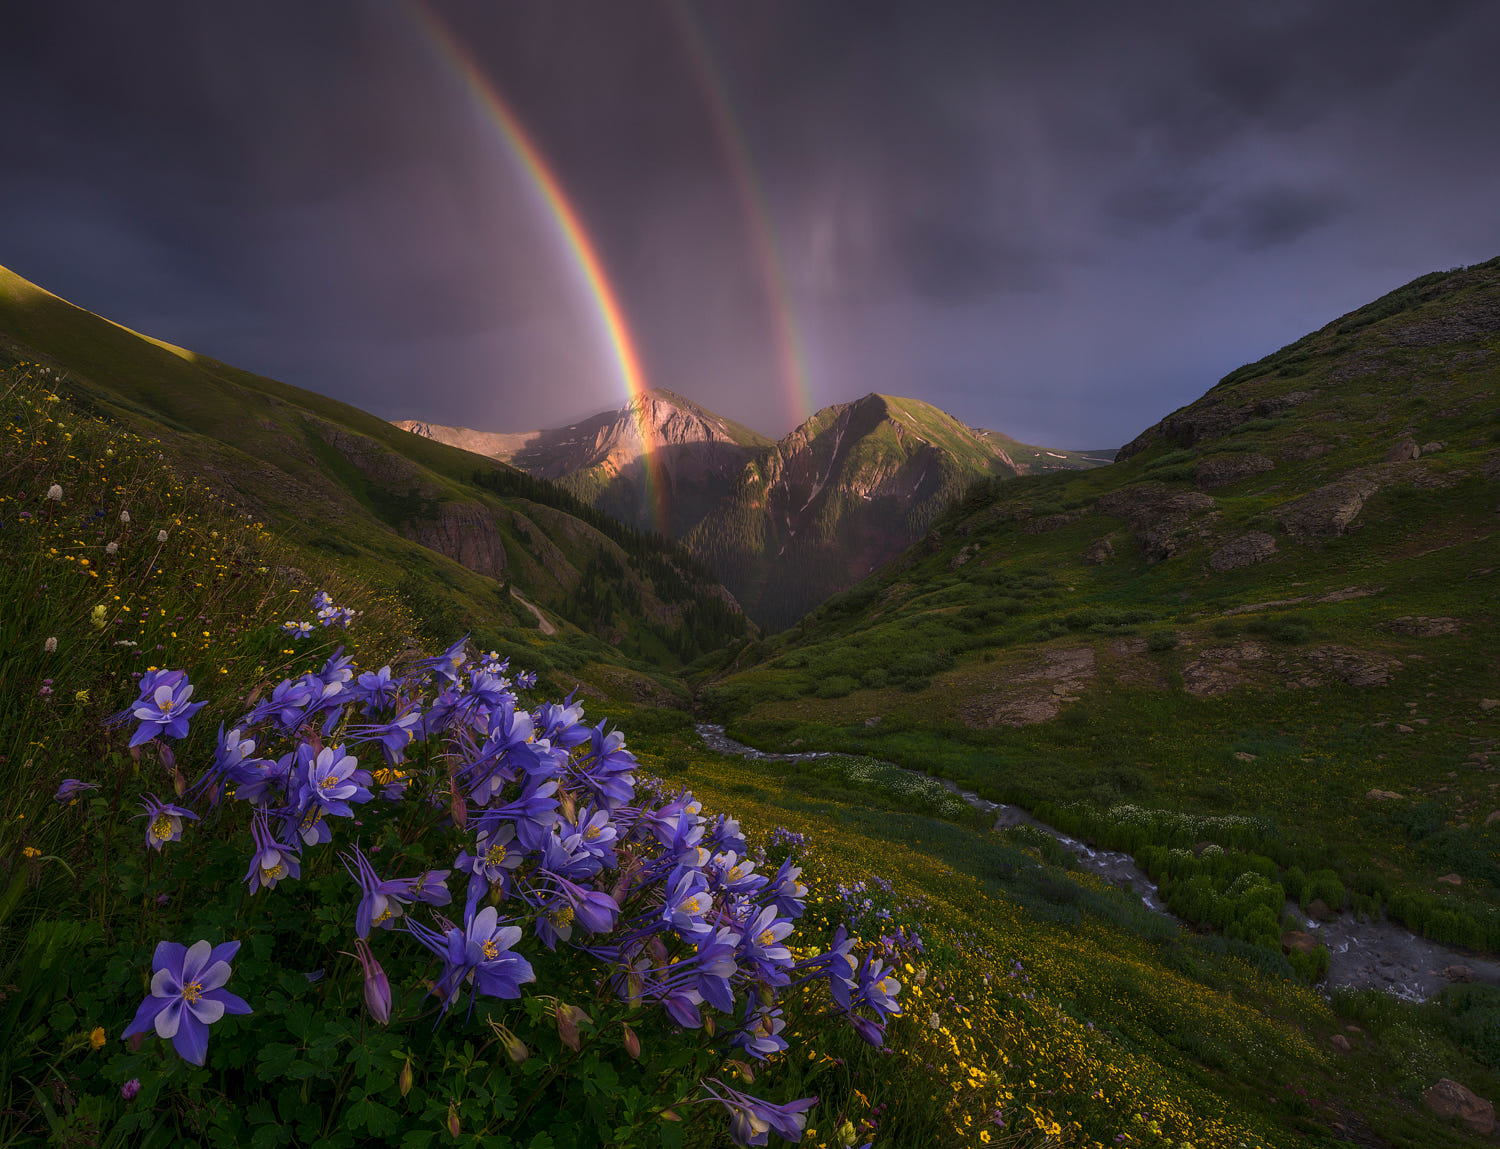
\includegraphics[width=0.9\columnwidth,height=5cm,keepaspectratio]{img/figure.jpg}
	\caption{Figura de ejemplo}%
	\label{fig:example-figure} %CHKTEX 24
\end{figure}

\begin{table*}[t]
	\centering
	\caption{Tabla de ejemplo con ancho de página completo}%
	\label{tbl:full-width-table} %CHKTEX 24
	\begin{tabularx}{0.9\textwidth}{X c c c c c c c c c}
	\toprule
	& Cabecera 1 & Cabecera 2 & Cabecera 3
	& Cabecera 4 & Cabecera 5 & Cabecera 6\\
	\midrule
	Fila 1 & a & b & c & d & e & f \\
	Fila 2 & g & h & i & j & k & l \\
	Fila 3 & m & n & o & p & q & r \\
	Fila 4 & s & t & u & v & w & x \\
	\bottomrule
	\end{tabularx}
\end{table*}
\subsection{Estilo y formato}
\label{sec:main-style}

La regla de oro en cuanto a estilo en \LaTeX{} es jamás modificar la plantilla que provee el editor.
Esto incluye
\begin{enumerate*}[label=\alph*\rpar]
	\item márgenes,
	\item espacio entre párrafos,
	\item espaciado de títulos,
	\item tamaño y tipo de letra,
	\item encabezado y pies de página
	y
	\item sangrías
\end{enumerate*}
entre otros.
Además, jamás deberán usarse primitivas de ajuste de espacio como \textcommand{vspace} y \textcommand{vskip}.

Todos los elementos de apoyo que incluyan (tablas, gráficos, código, algoritmos, diagramas, figuras, imágenes, etcétera) deben ir numerados y leyendados (ej.~con pie de foto o \textcommand{caption}), además de debidamente referidos en el texto, como la \Cref{tbl:column-width-table} y la \Cref{fig:example-figure}.
Se estila que los elementos gráficos lleven el pie de foto o leyenda en la parte inferior, mientras que los elementos de texto (tablas, código, algoritmos) la lleven en la parte superior.

\begin{table}[H]
	\centering
	\caption{Tabla de ejemplo con ancho de una columna}%
	\label{tbl:column-width-table} %CHKTEX 24
	\begin{tabularx}{0.9\columnwidth}{X c c c}
	\toprule
	& Cabecera 1 & Cabecera 2 & Cabecera 3 \\
	\midrule
	Fila 1 & a & b & c \\
	Fila 2 & d & e & f \\
	Fila 3 & g & h & i \\
	\bottomrule
	\end{tabularx}
\end{table}

Cuando agregue tablas, utilice las guías de estilo de \texttt{booktabs}, es decir los encabezados entre \texttt{toprule} y \texttt{midrule}, y \texttt{bottomrule} como línea inferior, sin delimitadores visibles verticales (rayas). Esto dará una apariencia más límpia.
Por otro lado, cuando las tablas tengan que presentar una gran cantidad de datos (recuerde presentar sólo lo relevante y prefiera vínculos a recursos en línea o use apéndices), estas podrían no caber en el espacio de una sola columna.
En estos casos utilice el entorno estrella delimitado por \textenviron{table*} para generar tablas del ancho de la página en documentos a doble columna, tal como ejemplifica la \Cref{tbl:full-width-table}.

En lo correspondiente a enumeraciones, para enumeraciones cortas se desaconseja el uso de listas ordenadas con un elemento por línea. En su lugar, y a fin de ahorrar espacio, se prefieren listas en línea, las cuales se pueden obtener importando el paquete \texttt{enumitem} con la opción \texttt{inline}, como se muestra en el \Cref{lst:inline-enum}.

\begin{lstlisting}[language={[LaTex]{TeX}},label={lst:inline-enum},caption={Enumeración en línea},captionpos=t]
\begin{enumerate*}[label=\alph*\rpar]
	\item elemento 1,
	\item elemento 2
	y
	\item elemento 3.
\end{enumerate*}
\end{lstlisting}

Otro aspecto importante es el de las citas y referencias.
En general, se espera que un documento cuente con al menos 70\% de contenido original, lo que deja entre un 20\% y 30\% del contenido para citas textuales y paráfrasis.
Es importante aclarar que el análisis y contraste de ideas se considera contenido original, por lo que referir a varias fuentes, comparar los puntos de vista, y realizar el proceso de síntesis de conclusiones no cuenta como plagio.

No obstante, el crédito siempre ha de darse de manera explícita.
En el caso de las citas textuales, éstas deberán ir entrecomilladas y seguidas de las referencias pertinentes mediante el comando \textcommand{cite}, cuando son cortas, o en un párrafo aparte con sangrías en ambos lados y letra cursiva cuando son largas.
Para evitar estos inconvenientes y lidiar con las tipografías que cada idioma requiere para el manejo de citas, se recomienda el uso del paquete \texttt{csquotes} que provee el comando \textcommand{enquote} para este propósito (véase \Cref{lst:enquote})~\Citep{Lehman2005csquotes}.

\begin{lstlisting}[language={[LaTex]{TeX}},label={lst:enquote},caption={Uso de enquote para entrecomillado de citas},captionpos=t]
\enquote{This package\dots include commands, environments, and user-definable \enquote{smart quotes} which dynamically adjust to their context. Quotation marks are switched automatically if quotations are nested andcan adjust to the current language}~\Citep{Lehman2005csquotes}.
\end{lstlisting}

Continuando con las citas, se aconseja el uso del paquete \textcommand{natbib} o algún otro manejador de referencias poderoso como \emph{biber}.
\texttt{natbib} ofrece comandos adicionales a \textcommand{cite} como los siguientes~\citep{Daly2006natbib}
\begin{itemize}
	\item\textbf{\textcommand{citep}:} Cita entre paréntesis, como en \emph{(Johnes et al.,~1990)}.
	\item\textbf{\textcommand{citep*}:} Cita entre paréntesis sin comprimir, como en \emph{(Johnes, Backer and Williams,~1990)}.
	\item\textbf{\textcommand{citet}:} Cita en texto, como en \emph{Johnes et al.~(1990)}.
	\item\textbf{\textcommand{citet*}:} Cita en texto sin comprimir, como en \emph{Johnes, Backer and Williams~(1990)}.
	\item\textbf{\textcommand{citeyear}:} Cita sólo el año de una publicación.
	\item\textbf{\textcommand{citeauthor}:} Cita sólo el autor de una publicación.
\end{itemize}

Además, \texttt{natbib} permite especificar capítulos y ofrece otra variedad de comandos para el control bibliográfico, y permite cambiar el estilo de referencia con facilidad entre APA, MLA, IEEE, etcétera.

\section{Conclusiones}
\label{sec:conclusions}
Todo trabajo debe cerrar con conclusiones, las cuales retoman los postulados o suposiciones iniciales y, tras una recapitulación de lo logrado, aprendido, o analizado, sintetizan los puntos más relevantes del trabajo.
Dicho de una manera simplista, es en las conclusiones donde se validan o refutan las hipótesis planteadas al principio con base en el trabajo realizado.

De manera similar, es en esta sección donde se reflexiona el alcance de lo conseguido y se proponen los siguientes pasos a seguir, qué falta por investigar, y que nuevas dudas, problemas o cuestionamientos plantea lo estudiado.

\section{Referencias}
\label{sec:references}
\nocite{*}
\bibliographystyle{unsrtnat}
\bibliography{references}

\end{document}
